%! app: TODOapp
%! outcome: TODOoutcome

\begin{center}
    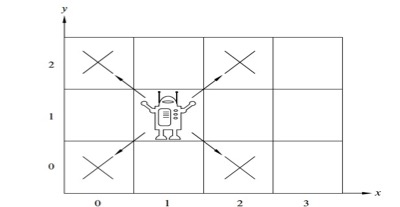
\includegraphics[width=3in]{../../resources/images/robot-grid.png}
\end{center}
    
{\bf Theorem}: A robot on an infinite 2-dimensional integer grid starts at $(0,0)$ and at each step moves
to diagonally adjacent grid point. This robot can / cannot {\footnotesize({\it circle one})} reach $(1,0)$.


{\bf Definition} The set of positions the robot can visit  $P$ is defined by:
\[
\begin{array}{ll}
    \textrm{Basis Step: } & (0,0) \in P \\
    \textrm{Recursive Step: } & \textrm{If } (x,y) \in P  \textrm{, then } 
    \phantom{(x+1, y+1), (x+1, y-1), (x-1, y-1), (x-1, y+1)} \textrm{ are also in } P
\end{array}
\]

{\it Example elements of $P$ are}:
\vspace{40pt}

{\bf Lemma}: $\forall (x,y) \in P( x+y \textrm{ is an even integer}~)$

{\it Why are we calling this a lemma?}


Proof of theorem using lemma: To show is $(1,0) \notin P$. Rewriting the lemma to explicitly 
restrict the domain of the universal, 
we have $\forall (x,y) ~(~ (x,y) \in P  \to (x+y \textrm{ is an even integer})~)$.  Since
the universal is true, 
$ (~ (1,0) \in P \to (1+0 \textrm{ is an even integer})~)$ is a true statement.
Evaluating the conclusion of this conditional statement: 
By definition of long division, since $1 = 0 \cdot 2 + 1$ (where $0 \in \mathbb{Z}$ and 
$1 \in \mathbb{Z}$ and $0 \leq 1 < 2$ mean that $0$ is the quotient and $1$ is the remainder), $1 ~\textrm{\bf mod}~ 2 = 1$ which is not $0$ 
so the conclusion is false.  A true conditional with a false conclusion must have a false hypothesis.
Thus, $(1,0) \notin P$, QED. $\square$

\vspace{20pt}

Proof of lemma by structural induction:

{\bf Basis Step}:

\vspace{100pt}


{\bf Recursive Step}:  Consider arbitrary $(x,y) \in P$.  To show is:
\[
(x+y \text{ is an even integer}) \to (\text{sum of coordinates of next position is even integer})
\]
Assume {\bf as the induction hypothesis, IH} that: 


\vspace{400pt}